%%\documentclass[sigconf,authordraft]{acmart}
\documentclass[sigconf,review,anonymous]{acmart}
%%
%% \BibTeX command to typeset BibTeX logo in the docs
\AtBeginDocument{%
  \providecommand\BibTeX{{%
    Bib\TeX}}}

\usepackage{etoolbox}
\makeatletter
\patchcmd{\@startsection}
  {\@afterindentfalse}
  {\@afterindenttrue}
  {}{}
\makeatother


\usepackage[utf8]{inputenc}
\usepackage{amsmath, amssymb}
\usepackage{geometry}
\usepackage{xeCJK}  % Optional: can be removed if no Chinese

\usepackage{graphicx}
\usepackage{hyperref}
\usepackage{multirow}
\usepackage[ruled,vlined,linesnumbered]{algorithm2e}
\DontPrintSemicolon
\RestyleAlgo{ruled}

\usepackage[colorinlistoftodos,prependcaption]{todonotes}
\usepackage{enumitem}
\usepackage{cancel,soul,ulem}

\newcommand{\stma}[1]{\todo[inline]{\textcolor{black}{#1}}}
\newcommand{\sta}[1]{\textcolor{blue}{#1}} 
\newcommand{\std}[1]{\textcolor{red}{\sout{#1}}}

\usepackage{mathtools}
\newcommand{\pluseq}{\mathrel{+}=}


% \newcommand{\stma}[1]{\todo[inline]{\textcolor{black}{}}}
% \newcommand{\sta}[1]{\textcolor{blue}{}} 
% \newcommand{\std}[1]{\textcolor{red}{\sout{}}}
%% Rights management information.  This information is sent to you
%% when you complete the rights form.  These commands have SAMPLE
%% values in them; it is your responsibility as an author to replace
%% the commands and values with those provided to you when you
%% complete the rights form.
\setcopyright{acmlicensed}
\copyrightyear{2018}
\acmYear{2018}
\acmDOI{XXXXXXX.XXXXXXX}
%% These commands are for a PROCEEDINGS abstract or paper.
\acmConference[ICSE '26]{Make sure to enter the correct
  conference title from your rights confirmation email}{April 12--18,
  2026}{Rio de Janeiro, Brazil}
%%
%%  Uncomment \acmBooktitle if the title of the proceedings is different
%%  from ``Proceedings of ...''!
%%
%%\acmBooktitle{Woodstock '18: ACM Symposium on Neural Gaze Detection,
%%  June 03--05, 2018, Woodstock, NY}
\acmISBN{978-1-4503-XXXX-X/2018/06}


%%
%% Submission ID.
%% Use this when submitting an article to a sponsored event. You'll
%% receive a unique submission ID from the organizers
%% of the event, and this ID should be used as the parameter to this command.
%%\acmSubmissionID{123-A56-BU3}

%%
%% For managing citations, it is recommended to use bibliography
%% files in BibTeX format.
%%
%% You can then either use BibTeX with the ACM-Reference-Format style,
%% or BibLaTeX with the acmnumeric or acmauthoryear sytles, that include
%% support for advanced citation of software artefact from the
%% biblatex-software package, also separately available on CTAN.
%%
%% Look at the sample-*-biblatex.tex files for templates showcasing
%% the biblatex styles.
%%

%%
%% The majority of ACM publications use numbered citations and
%% references.  The command \citestyle{authoryear} switches to the
%% "author year" style.
%%
%% If you are preparing content for an event
%% sponsored by ACM SIGGRAPH, you must use the "author year" style of
%% citations and references.
%% Uncommenting
%% the next command will enable that style.
%%\citestyle{acmauthoryear}


%%
%% end of the preamble, start of the body of the document source.
\begin{document}

%%
%% The "title" command has an optional parameter,
%% allowing the author to define a "short title" to be used in page headers.
\title{From Generation to Reasoning: Chain-of-Thought Guided Merge Conflict Resolution}

%%
%% The "author" command and its associated commands are used to define
%% the authors and their affiliations.
%% Of note is the shared affiliation of the first two authors, and the
%% "authornote" and "authornotemark" commands
%% used to denote shared contribution to the research.
\author{Ben Trovato}
\authornote{Both authors contributed equally to this research.}
\email{trovato@corporation.com}
\orcid{1234-5678-9012}
\author{G.K.M. Tobin}
\authornotemark[1]
\email{webmaster@marysville-ohio.com}
\affiliation{%
  \institution{Institute for Clarity in Documentation}
  \city{Dublin}
  \state{Ohio}
  \country{USA}
}

\author{Lars Th{\o}rv{\"a}ld}
\affiliation{%
  \institution{The Th{\o}rv{\"a}ld Group}
  \city{Hekla}
  \country{Iceland}}
\email{larst@affiliation.org}

\author{Valerie B\'eranger}
\affiliation{%
  \institution{Inria Paris-Rocquencourt}
  \city{Rocquencourt}
  \country{France}
}

\author{Aparna Patel}
\affiliation{%
 \institution{Rajiv Gandhi University}
 \city{Doimukh}
 \state{Arunachal Pradesh}
 \country{India}}

\author{Huifen Chan}
\affiliation{%
  \institution{Tsinghua University}
  \city{Haidian Qu}
  \state{Beijing Shi}
  \country{China}}

\author{Charles Palmer}
\affiliation{%
  \institution{Palmer Research Laboratories}
  \city{San Antonio}
  \state{Texas}
  \country{USA}}
\email{cpalmer@prl.com}

\author{John Smith}
\affiliation{%
  \institution{The Th{\o}rv{\"a}ld Group}
  \city{Hekla}
  \country{Iceland}}
\email{jsmith@affiliation.org}

\author{Julius P. Kumquat}
\affiliation{%
  \institution{The Kumquat Consortium}
  \city{New York}
  \country{USA}}
\email{jpkumquat@consortium.net}

%%
%% By default, the full list of authors will be used in the page
%% headers. Often, this list is too long, and will overlap
%% other information printed in the page headers. This command allows
%% the author to define a more concise list
%% of authors' names for this purpose.
\renewcommand{\shortauthors}{Trovato et al.}

%%
%% The abstract is a short summary of the work to be presented in the
%% article.
\begin{abstract}
Merge conflicts have become a critical bottleneck in version control systems, significantly hindering development efficiency, and typically rely on manual, time-consuming processing.
In recent years, learning-based methods have transformed the solution of merge conflicts from a classification problem to a generative task, directly generating post-conflict code by sequentially generating code tokens. Although this approach overcomes certain limitations of classification methods (e.g., the inability to introduce new code tokens), we observe that relying solely on the conflicting code for direct generation makes it difficult to effectively handle complex conflict scenarios that require the integration of non-trivial semantics and distributed modifications. 
To address this, this paper redefines merge conflict resolution as a reasoning task and proposes \textbf{MergeCoT}, an automated resolution framework based on Chain-of-Thought (CoT) prompting with Large Language Models (LLMs). 
Specifically, we design a simple Domain-Specific Language (DSL), introducing an Edit Script (ES) to structurally represent conflict information and guide the reasoning process. 
We then automatically construct a training dataset with explicit reasoning traces using a two-stage data generation pipeline that leverages both DSL and ES representations.
Experimental results on this dataset show that MergeCoT significantly outperforms the current state-of-the-art (SOTA) techniques in terms of precision and accuracy. 
The accuracy on Java reached 73.8\% (an absolute improvement of 6.1\%). Furthermore, experiments on various programming languages demonstrate MergeCoT’s superior multilingual versatility and cross-language
generalisation ability. Additional ablation studies validate the critical role of the ES and CoT mechanisms in enhancing performance.

\end{abstract}

%%
%% The code below is generated by the tool at http://dl.acm.org/ccs.cfm.
%% Please copy and paste the code instead of the example below.
%%
% \begin{CCSXML}
% <ccs2012>
%  <concept>
%   <concept_id>00000000.0000000.0000000</concept_id>
%   <concept_desc>Do Not Use This Code, Generate the Correct Terms for Your Paper</concept_desc>
%   <concept_significance>500</concept_significance>
%  </concept>
%  <concept>
%   <concept_id>00000000.00000000.00000000</concept_id>
%   <concept_desc>Do Not Use This Code, Generate the Correct Terms for Your Paper</concept_desc>
%   <concept_significance>300</concept_significance>
%  </concept>
%  <concept>
%   <concept_id>00000000.00000000.00000000</concept_id>
%   <concept_desc>Do Not Use This Code, Generate the Correct Terms for Your Paper</concept_desc>
%   <concept_significance>100</concept_significance>
%  </concept>
%  <concept>
%   <concept_id>00000000.00000000.00000000</concept_id>
%   <concept_desc>Do Not Use This Code, Generate the Correct Terms for Your Paper</concept_desc>
%   <concept_significance>100</concept_significance>
%  </concept>
% </ccs2012>
% \end{CCSXML}

% \ccsdesc[500]{Do Not Use This Code~Generate the Correct Terms for Your Paper}
% \ccsdesc[300]{Do Not Use This Code~Generate the Correct Terms for Your Paper}
% \ccsdesc{Do Not Use This Code~Generate the Correct Terms for Your Paper}
% \ccsdesc[100]{Do Not Use This Code~Generate the Correct Terms for Your Paper}

%%
%% Keywords. The author(s) should pick words that accurately describe
%% the work being presented. Separate the keywords with commas.
\keywords{Merge Conflict Resolution, Large Language Model, Chain of Thought}
%% A "teaser" image appears between the author and affiliation
%% information and the body of the document, and typically spans the
%% page.


% \received{20 February 2007}
% \received[revised]{12 March 2009}
% \received[accepted]{5 June 2009}

%%
%% This command processes the author and affiliation and title
%% information and builds the first part of the formatted document.
\maketitle

\section{INTRODUCTION}
In large software projects, collaborative development models significantly improve project delivery efficiency through task decomposition and parallel development. Developers typically rely on version control systems such as Git, working on independent feature branches and merging changes into the main branch through pull requests, followed by code reviews to complete the merge~\cite{1}. However, while this model improves development efficiency, it also introduces the potential risk of merge conflicts. Studies show that approximately 12\% of project commit records involve merge operations, with nearly 46\% of these merge commits encountering conflicts~\cite{2}. Conflicts are likely to arise when multiple developers make parallel modifications to the same code area and attempt to merge their changes. The conflict resolution process not only interrupts the developers' original workflow but also requires them to deeply understand the semantic logic and business context of the conflicting code, as well as devise reasonable merge strategies based on project specifications. During this process, developers often need to collaborate with team members, making the overall task highly complex, time-consuming, and error-prone~\cite{3}.

Currently, mainstream version control systems, represented by Git, commonly use the diff3 algorithm to detect conflicts during the merge process~\cite{4}. This algorithm compares two branch versions, A and B, with their common ancestor version O, identifies differences relative to O, and aligns these differences into several conflict slots.
When A and B both contain modifications relative to O in the same slot (e.g., the same line), a conflict is detected, and manual intervention is required to complete the merge. To reduce the manual burden on developers during conflict resolution, researchers have conducted extensive studies in the field of automatic merge conflict resolution~\cite{5, 6, Sousa, 8}. This task is typically defined as: given the conflicting versions A, B, and their common ancestor O, automatically generate a semantically correct merged result.

Existing automatic conflict resolution methods can mainly be classified into three types: unstructured methods~\cite{9}, structured methods~\cite{10, 11, 6}, and semi-structured methods~\cite{13}. Unstructured methods rely on text similarity to identify conflict locations but cannot perform automatic fixes. Structured and semi-structured methods model the conflict using Abstract Syntax Trees (AST), which, while more accurate in semantic understanding, often suffer from high computational overhead and strong dependencies on specific programming languages, limiting their applicability in real-world scenarios.

In recent years, deep learning-based conflict resolution methods have gradually emerged, leveraging historical data to learn conflict patterns and corresponding resolution strategies, showing high processing efficiency and a certain degree of generalisation ability. 

Among them, one type of these methods models conflict resolution as a classification problem~\cite{mergebert}, aiming to select or combine existing content from conflicting versions to generate a solution. 
Such methods cannot generate new tokens—that is, new code elements not present in the input, making it difficult to meet real-world needs such as introducing new logic (e.g., adding functions to integrate two versions). Moreover, they often ignore the contextual relationships between tokens when handling line-level conflicts, which leads to incomplete or inconsistent results.
Another type of method models conflict resolution as a generative task~\cite{mergegen}, capable of generating new tokens outside the input range, offering greater flexibility. However, this method still faces two major issues: first, when handling complex conflicts, it may simply concatenate the content of the two branches, leading to logical or syntactic errors in the generated code; second, the model is highly dependent on specific datasets and must be trained separately for different programming languages, still showing limited generalisation ability. Furthermore, whether conflict resolution is modelled as a classification problem or a generative task, most existing methods focus only on generating the final resolution, lacking modelling and explanation of the intermediate reasoning process, and thus exhibiting significant limitations in terms of explainability.

To address the above challenges, we propose MergeCoT, an automated merge conflict resolution method based on Chain-of-Thought (CoT) guidance. Chain-of-thought prompting encourages models to generate intermediate reasoning steps before producing final answers. Wei et al. demonstrated that incorporating Chain-of-Thought reasoning can significantly enhance a model’s performance on tasks that require complex reasoning~\cite{cot}.

We first design a concise Domain-Specific Language (DSL) that structurally and compactly represents conflict information while preserving completeness.
We define an Edit Script (ES) as an ordered sequence of DSL statements, each encoding a specific edit from one of the conflicting branches.
Compared with prompting directly on raw conflict text, an ES provides a normalised focus signal that helps the model attend to the edits in each branch. Based on this representation, we construct a dataset paired with effective thought chains.

We perform a systematic evaluation of MergeCoT across multiple programming languages. Experimental results show that MergeCoT significantly outperforms current SOTA methods in terms of both precision and accuracy. 

Further ablation studies validate MergeCoT’s excellent generalisation ability in multilingual environments and fully demonstrate the key role of the ES and CoT mechanisms in improving model performance.
 \medskip
 \noindent

The main contributions of this paper are as follows:
\begin{itemize}
\item Innovative Task Modelling. We redefine merge conflict resolution as a reasoning task, distinguishing it from previous approaches that treat it as a classification or generative problem. This modelling approach introduces the CoT reasoning mechanism, simulating the multi-step thought process that developers go through when resolving merge conflicts, thereby improving the rationale and explainability of the solution.
\item ES Prompting Mechanism. We design an ES prompting mechanism based on DSL that simplifies conflict information while retaining the semantic integrity of changes in each branch, significantly improving the quality and context coverage of the generated thought chains.
\item Data Construction Method. We propose an automated method for constructing thought chain datasets, which enhances data quality through a two-stage process: “free generation” and “reasoning-based filtering.” Experimental results show that this method allows approximately 90\% of the original conflict samples to have clearly structured, semantically consistent thought chains, significantly reducing the manual labelling cost. 
\item Extensive Experimental Validation. We systematically evaluate MergeCoT on multiple mainstream programming language datasets. The results demonstrate that the method outperforms the current SOTA in both precision and accuracy, while showcasing excellent multilingual versatility and generalisation capability.
\end{itemize}

Additionally, all related resources—including the code, training dataset, and trained LoRA adapter checkpoints—are open-sourced to facilitate future research and practical applications. 
These are available at \url{https://anonymous.4open.science/r/MergeCoT-AF6D/readme.md}.



\section{MOTIVATION}

Existing deep learning-based merge conflict resolution methods, such as MergeBERT, model conflicts as a classification task but perform poorly in scenarios that require introducing new tokens, as they cannot generate content beyond the input range~\cite{mergebert}. 
To address this limitation, the current SOTA method MergeGen introduces a structural and fine-grained conflict-aware representation and uses an autoregressive approach to generate solutions token by token~\cite{mergegen}, achieving significant improvements in handling complex conflicts. 
However, whether in classification or generative models, these methods essentially treat conflict information as a black-box input and directly produce solutions, lacking modelling of the intermediate reasoning process. This results in poor explainability of the generated outcomes, which fails to meet developers’ needs for decision transparency. This section will further analyse the limitations of existing methods and illustrate their shortcomings in handling complex conflicts with specific examples.

\subsection{Limitation 1: Handling Complex Conflicts}
\begin{figure}[b]
    \centering
    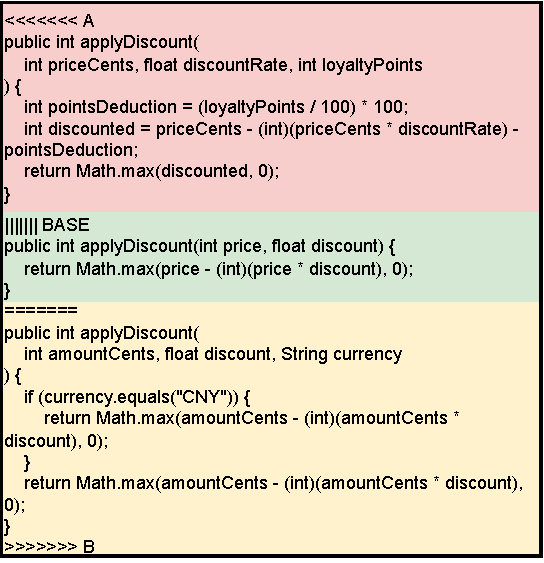
\includegraphics[width=1\linewidth]{Figures/Conflict example diagram.pdf}
    \caption{Conflict example.}
    \label{fig:Conflict example}
\end{figure}

\autoref{fig:Conflict example} shows a typical merge conflict example, where the standard diff3 algorithm generates the merge result.
The conflict region is delimited by the markers \verb|<<<<<<<| and \verb|>>>>>>>|. Inside the block, \verb|<<<<<<<|\ A marks content from branch A, \verb+|||||||+\ BASE shows the common ancestor version O, \verb|=======| separates the two sides, and \verb|>>>>>>>|\ B closes the block with content from branch B. In this example, branch A introduces a points redemption mechanism based on the original discount logic, replacing price and discount in the base version with priceCents and discountRate; branch B renames the price variable to amountCents, adds a currency parameter, and includes special logic for handling "CNY."

The ideal conflict resolution should integrate both changes, using the more refined unit representation (cents) while preserving the points redemption feature and the currency determination logic.  However, existing methods—whether classification-based MergeBERT or generative MergeGen—often fail to understand the intent behind changes in each branch deeply and tend to perform superficial concatenation, leading to issues such as mixed variables and logical omissions.
For example, priceCents and amountCents in~\autoref{fig:Conflict example} actually represent the same concept, and if the model cannot recognise this semantic equivalence and combines them based on surface-level text, it may use different variable names in the merged result, causing syntax errors or semantic confusion. Therefore, when faced with conflicts involving structural differences and complex semantic changes, existing methods lack the necessary reasoning capabilities and struggle to generate semantically consistent and functionally complete solutions.

\subsection{Limitation 2: Lack of Explainability}

Another major limitation of deep learning-based merge conflict resolution methods is the lack of explainability in the generated results. 
Existing models typically accept conflicting code as input and produce a merged result directly, without explaining the generation process. 
As a result, their behaviour is more like a black-box recommendation for developers. 

Because developers cannot understand the model’s decision-making basis, they often find it difficult to trust and adopt such automatic merge results. If the model could provide a readable reasoning process alongside the generated solution, gradually demonstrating its decision-making logic at each step, it would not only help developers verify the rationale behind the result but also significantly increase their trust in the model’s behaviour, thereby improving the adoption of automated merge technologies.

\subsection{Limitation 3: Limited Generalisation Ability}

Currently, both classification-based and generative methods generally rely on specific programming language datasets. When facing different languages or cross-project scenarios, additional model training or fine-tuning is often required, leading to weak cross-language transferability and limited generalisation. 
In contrast, introducing a CoT reasoning mechanism helps the model understand the general logic of conflict resolution at a deeper level. By simulating the reasoning process of human developers when handling conflicts—first analysing the changes in each branch, understanding the functional intentions behind them, and then manually synthesising a merged solution that meets both sides’ expectations—the model can learn abstract conflict resolution patterns from data, allowing it to transcend specific language and syntax dependencies.

To achieve this goal, this paper proposes MergeCoT, which guides the model to generate intermediate reasoning steps, thereby enhancing its ability to understand the causes of conflicts and construct resolution paths. 
This leads to the generation of more accurate, interpretable, and highly generalised (i.e., transferable across languages/projects) merge results.

\section{METHOD}
This section presents a detailed description of the proposed method, MergeCoT, with an overview of the process illustrated in~\autoref{fig:MergeCoT}.
MergeCoT is based on a decoder-only Transformer architecture, and its framework consists of two core components: (i) \textit{Edit Script Prompting}. This module defines how to express conflict information in a structured manner to guide the model through step-by-step reasoning; (ii) \textit{CoT Dataset Construction}. This part aims to construct a dataset that contains the intermediate reasoning process for training the model, thereby enhancing its explainability and generalisation ability. Section A introduces the design and construction of ES Prompting, while Section B provides a detailed explanation of how the CoT dataset, including thought chains, is automatically constructed.
\begin{figure*}[t]
    \centering
    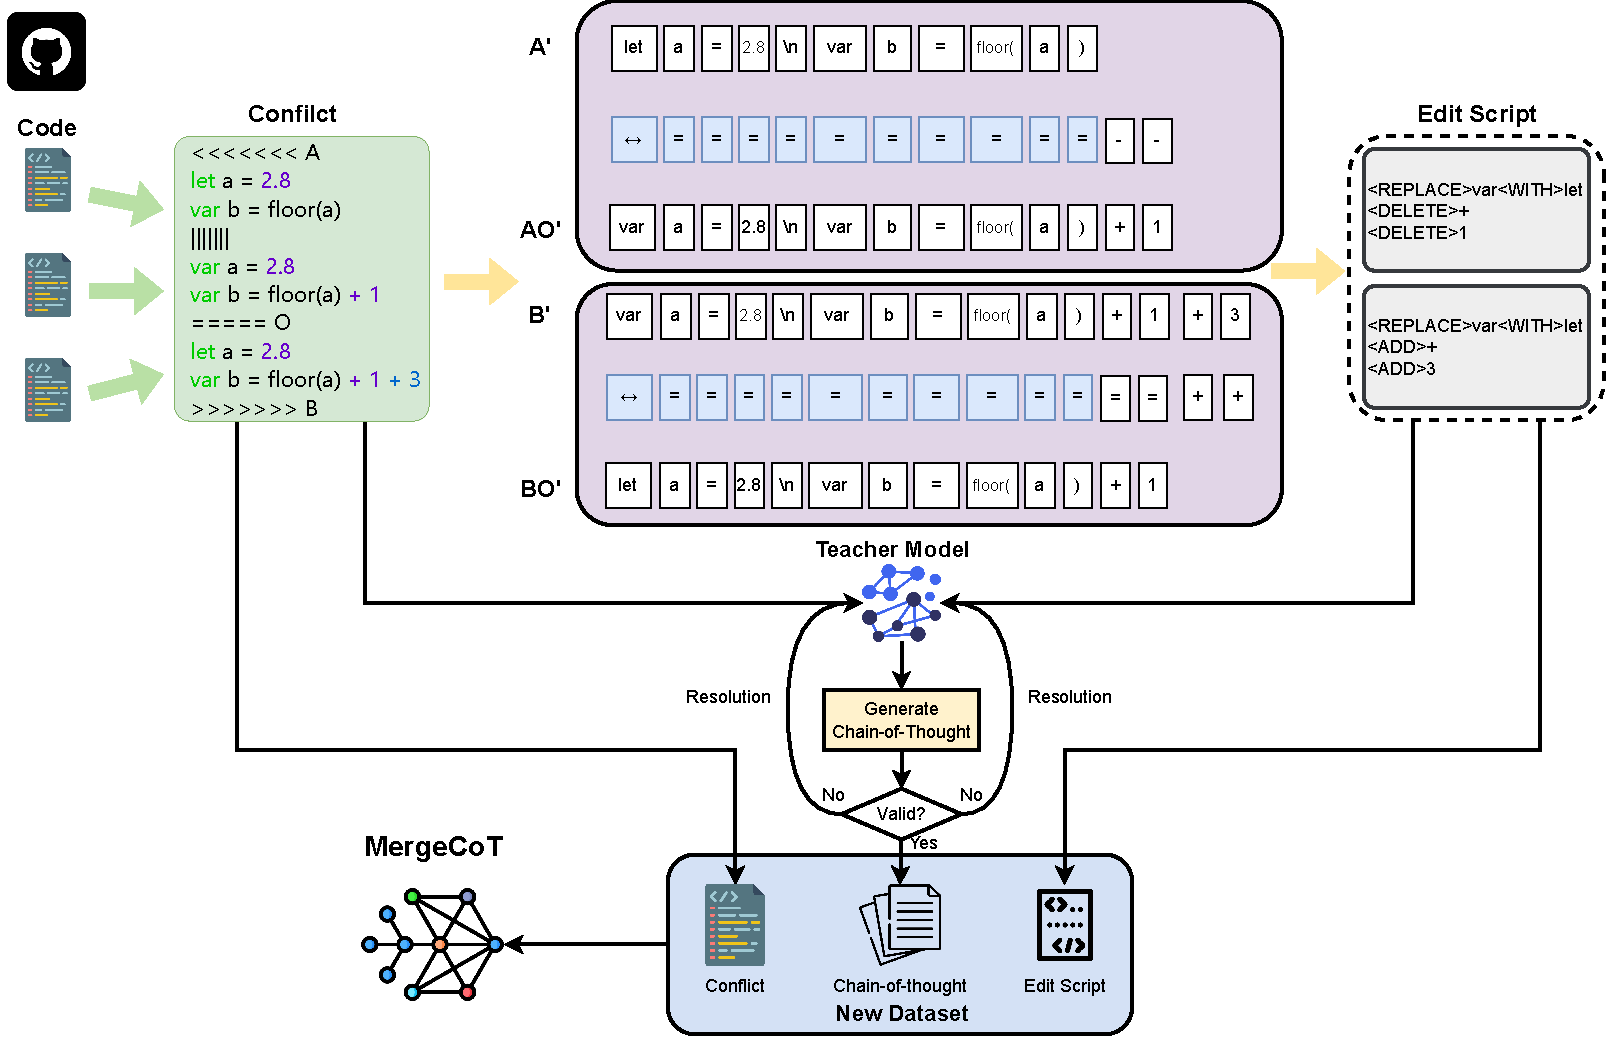
\includegraphics[width=1\linewidth]{Figures/MergeCoT.pdf}
    \caption{The overview of MergeCoT.}
    \label{fig:MergeCoT}
\end{figure*}
\subsection{Edit Script Prompting}
CoT prompting is a technique that guides large language models to output intermediate reasoning steps before generating the final result~\cite{cot}.
It has been shown to significantly improve model performance in tasks such as arithmetic calculations and commonsense reasoning. 

In the context of merge conflicts, we expect the model first to produce a series of logical reasoning steps that explain the conflict resolution process before generating the final merged code.
However, directly applying CoT in code conflict scenarios presents challenges: the model may struggle to identify the relevant change locations or may overlook key differences. 
If only generalised prompts (e.g., "Please explain how to merge") are given, the resulting thought chains often lack completeness and focus. 
To address this, this paper introduces an ES Prompting Strategy that explicitly expresses the differences between branches and the base version in a structured way, guiding the model to perform targeted reasoning.

Previous research~\cite{ltre} proposed a concise representation method for encoding two-way diffs. This method uses a standard deterministic diff algorithm and represents the generated pairwise alignment results as an automatically encoded fixed-dimensional vector. The edit sequence generated from a single two-way alignment primarily includes the following types of editing operations: 
$=$ indicates that two tokens are the same, 
$+$ indicates an insertion, 
$-$ indicates a deletion, and 
$\leftrightarrow$ indicates a replacement. 
Additionally, the method introduces two special tokens: 
$\phi$ represents padding, and $|$ represents a newline.
However, these edit sequences only capture the types of edit operations and ignore the specific tokens involved in the edits (except for newline tokens).

Considering that conflict code in real-world scenarios may be relatively long, we designed a concise DSL to represent the editing operations between branches and the base version. This language includes the following three basic instructions:
\begin{itemize}
    \item \texttt{<ADD> X}: Indicates that $X$ is newly added content (present in the branch but missing in the base version).
    \item \texttt{<DELETE> X}: Indicates that $X$ is deleted content (present in the base version but missing in the branch).
    \item \texttt{<REPLACE> X <WITH> Y}: Indicates that $X$ in the base version has been replaced with $Y$ in the branch.
\end{itemize}
Here, $X$ and $Y$ denote concrete token sequences (possibly multi-token substrings) extracted from the corresponding base/branch spans under a deterministic tokenisation; they are not placeholders. When the same token string appears multiple times, $X$ and $Y$ refer to the specific occurrence within the aligned span indicated by the ES.

This DSL representation not only simplifies the conflict information but also provides clear contextual guidance for generating thought chains.

Algorithm~\ref{alg:build-es} presents the procedure for constructing an Edit Script, a concise and structured representation of conflict information capturing the fine-grained edits between two token sequences—the original version $O$ and the revised branch $A$. Specifically, we first segment the input sequences into a series of operation blocks (equal, insert, delete, replace) using dynamic sequence alignment (denoted as \textsc{DiffBlocks}). Each block is then processed to produce aligned token sequences $O'$ and $A'$. For insertions and deletions, placeholders ($\varnothing$) are inserted to maintain alignment. For replacement blocks, the shorter segment is padded with placeholders using a token-level alignment procedure (\textsc{Align}). Finally, these aligned segments are translated into explicit edit operations $\Delta_{AO}$, providing a clear semantic interpretation of the differences. The resulting ES effectively guides downstream reasoning or generative tasks by highlighting precisely what has changed between versions.

\begin{algorithm}[t]
\caption{\textsc{Build-ES}: Generate Edit-Script DSL from two token sequences}
\label{alg:build-es}
\KwData{$A$ (revised tokens), $O$ (original tokens)}
\KwResult{$(A', O', \Delta_{AO})$}
$A' \gets [\,]$; $O' \gets [\,]$; $\Delta_{AO} \gets [\,]$\;
$\mathcal{B} \gets \textsc{DiffBlocks}(O,A)$  \tcp*[r]{equal / insert / delete / replace spans}
\ForEach{$(tag,\;O[i{:}i'),\;A[j{:}j')) \in \mathcal{B}$}{
  \uIf{$tag = \textsc{Equal}$}{
    append $A[j{:}j')$ to $A'$, $O[i{:}i')$ to $O'$; no op emitted\;
  }
  \uElseIf{$tag = \textsc{Insert}$}{
    append $A[j{:}j')$ to $A'$, $\varnothing^{|j'-j|}$ to $O'$;\;
    $\Delta_{AO} \pluseq \textsc{Add}(A[j{:}j'))$\;
  }
  \uElseIf{$tag = \textsc{Delete}$}{
    append $\varnothing^{|i'-i|}$ to $A'$, $O[i{:}i')$ to $O'$;\;
    $\Delta_{AO} \pluseq \textsc{Delete}(O[i{:}i'))$\;
  }
  \Else(\tcp*[h]{replace}) {
    $(O_s, A_s) \gets \textsc{AlignByLength}(O[i{:}i'), A[j{:}j'))$ \tcp*{pad shorter w/ $\varnothing$}
    append $A_s$ to $A'$, $O_s$ to $O'$;\;
    $\Delta_{AO} \pluseq \textsc{Replace}(O_s, A_s)$\;
  }
}
\Return $(A', O', \Delta_{AO})$\;
\end{algorithm}

The specific operations include four types:
When tokens are equal ($\textit{equal}$), the corresponding token is directly appended to the aligned sequence, and no additional edit operation is recorded.
When a replacement ($\textit{replace}$) occurs, the corresponding tokens at the aligned positions are compared one by one, and the detailed replacement operation is recorded.
When an insertion (\textit{insert}) occurs in the revised sequence A, the new token is appended to A', and recorded as an ADD operation.
When a deletion (\textit{delete}) occurs in the original sequence O, the deleted token is recorded as a DELETE operation.

The final output is a detailed change operation set $\Delta_{AO}$, $\Delta_{BO}$, which together form an ES for the conflict. An example of an ES for a conflict is shown in~\autoref{fig:MergeCoT}. This fine-grained token-level alignment helps with subsequent in-depth analysis and modelling of text changes.

We adopt structured editing techniques for two main benefits: (1) explicitly highlighting the changes in each branch, ensuring that the model focuses on every addition, deletion, and replacement; and (2) simplifying the conflict changes significantly reduces the cognitive and token burden on the model. The DSL we define abstracts away unchanged content, making it more compact than the full code versions. Essentially, we provide the model with a change map to guide its reasoning.

For the Transformer model, the ES can be viewed as an anchor point for the attention mechanism and a logical framework for the reasoning process. The self-attention mechanism allows the model to focus on the relevant parts of the ES during the generation of reasoning or code, providing factual evidence for the reasoning process. We train the model using a multitask learning approach, forcing the model to follow a structured reasoning process: given $(X, \Delta)$, the model first generates a CoT, and then, based on $(X, \Delta, \text{CoT})$, generates the final merged code. The loss function for the model is as follows:

\begin{equation}
\mathcal{L} = -\Big(\underbrace{\sum_{t} \log P_\theta(c_t \mid X, \Delta, c_{<t})}_{\text{CoT generation loss}} + \underbrace{\sum_{s} \log P_\theta(y_s \mid X, \Delta, \text{CoT}, y_{<s})}_{\text{Final code generation loss}}\Big)
\end{equation}


where $c_t$ represents a token in the CoT, and $y_s$ represents a token in the merged code. Essentially, we supervise both the intermediate reasoning process and the final answer generation, guiding the model to learn the underlying reasoning flow, thus achieving the correct merge. The reasoning process (rationale) and the answer are jointly decoded as a sequence, simplifying the training process. During the reasoning generation phase, we can choose to display the CoT to the user or keep it for internal use (i.e., for guiding the model’s hidden states).

\subsection{Construction of the CoT Dataset}\label{sec: CoT}

In the previous sections, we have detailed the concept of edit-aware CoT, but obtaining sufficient training data containing real CoT remains a significant challenge. Prior to any CoT generation, we first partition the corpus into disjoint training, validation, and test splits. The two-stage CoT generation pipeline is then applied only on the training split to build the curated CoT corpus; the validation split is used for model selection and the test split is reserved for final evaluation. 
Although examples containing conflicts and resolved code are easy to obtain from code repositories, these examples do not contain explicit reasoning processes (i.e., CoT). 
Manually annotating CoT for thousands or even tens of thousands of conflicts is clearly not feasible. 
In the STaR (Self-Taught Reasoner) method proposed by Zelikman et al.~\cite{star}, the model is trained on a small-scale seed set and then bootstraps the CoT on a large-scale unlabelled dataset, generating reasoning and answers, and continuing training on successful samples. 
We made the following three improvements to this method to increase the quality and quantity of CoT data:

\textbf{Using a stronger teacher model to generate candidate CoT.} We use Qwen3 32B as the teacher model, which has powerful code understanding and generation capabilities with high efficiency. In addition to its strong benchmark performance among open-source models, we choose Qwen3 32B because it is open-source and supports reliable local deployment; at our scale, relying on commercial API access would be prohibitively expensive. We input each conflict (including the ES prompt) into the teacher model and ask it to output the CoT and the merged result.

\textbf{Adding a rationalisation stage for incorrect answers.} Some merges generated by the teacher model are correct, while others are incorrect. For incorrect merges, we do not discard them directly. Instead, we provide the correct merged code (from the training set) and ask the teacher model to explain this correct answer. 
Intuitively, even if the model initially cannot generate the correct reasoning, it can still produce reasonable reasoning after knowing the correct answer—this is abductive reasoning.
% \stma{or....answer-an instance of abductive reasoning.}

\textbf{For each merge conflict, we generate $K$ CoTs and their corresponding answers by adjusting the temperature.} Since large-scale language models (LLMs) can generate multiple answers, increasing the number of generated answers improves the probability of success in the final result. This method helps increase the diversity of the dataset. In our experiments, we set $K=3$, which balances the available computational resources with the theoretical benefits of larger self-consistency-style sampling budgets~\cite{wang2022selfconsistencyArXiv}.

\begin{algorithm}[t]
\caption{\textsc{CoT Generation}}\label{alg2}
\KwIn{$T$: teacher LLM\\
      $\mathcal{D} = \{(x_i, y_i)\}_{i=1}^{D}$: merge-conflict dataset\\
      $K$: number of generations per stage}
\KwOut{$\mathcal{C}$: curated CoT corpus}
\BlankLine
$\mathcal{C} \gets \emptyset$\;
\ForEach{$(x, y) \in \mathcal{D}$}{
  \tcp{Stage 1: unconditional generation}
  $\mathcal{G}_1 \gets \{\, (r_j, \hat{y}_j) \leftarrow T(x) \mid j = 1 \dots K \,\}$\;
  \uIf{$\exists\,j : \hat{y}_j = y$}{
    \ForEach{$(r_j, \hat{y}_j) \in \mathcal{G}_1 \,\mid\, \hat{y}_j = y$}{
      $\mathcal{C} \gets \mathcal{C} \cup \{ (x, r_j, y) \}$\;
    }
  }
  \Else{
    \tcp{Stage 2: hinted generation}
    $x^{\text{hint}} \gets \texttt{add\_hint}(x, y)$\;
    $\mathcal{G}_2 \gets \{\, (r^{\text{hint}}_j, \hat{y}^{\text{hint}}_j) \leftarrow T(x^{\text{hint}}) \mid j = 1 \dots K \,\}$\;
    \ForEach{$(r^{\text{hint}}_j, \hat{y}^{\text{hint}}_j) \in \mathcal{G}_2 \,\mid\, \hat{y}^{\text{hint}}_j = y$}{
      $\mathcal{C} \gets \mathcal{C} \cup \{ (x, r^{\text{hint}}_j, y) \}$\;
    }
  }
}
\Return $\mathcal{C}$\;
\end{algorithm}

As shown in the algorithm~\ref{alg2}, our dataset generation process is divided into two stages:

\textbf{Stage 1 (Free Generation):} Given a merge conflict dataset $\mathcal{D}={(x_i,y_i)}_{i=1}^{D}$, for each conflict sample $x_i$, we first input $x_i$ (with the ES prompt) into the model and ask it to output $K$ CoTs and merged code (where $K$ is the number of sampled candidates per instance). If the generated merged code matches the real merge result $y_i$ (verified via strict string matching), the pair $(r_i, y_i)$ is adopted as part of the new training set, where $r_i$ denotes the selected reasoning trace (CoT) corresponding to $x_i$.

\textbf{Stage 2 (Rationalisation):} For conflicts where Stage 1 failed to generate the correct merged code, we incorporate the real answer $y_i$ as a hint into the conflict instance and ask the model to provide a step-by-step reasoning process, ultimately generating $K$ CoTs that match the answer. 
The resulting CoTs, which match the real answer, are added to the new training set as $(r_i, y_i)$.

Through these two stages, we ultimately obtain a high-quality CoT dataset $\mathcal{C}={(x_i, r_i, y_i)}$, where each CoT $r_i$ is consistent with the real merge conflict solution $y_i$. This method ensures the accuracy and consistency of the CoT in the dataset, while also considering the diversity of the data.

This method is highly efficient. Although in the worst case, each instance may require up to $2K$ calls to the teacher model, in practice, most data will terminate early in Stage 1 (e.g., 49.5\% of Java data finishes in Stage 1), significantly reducing the overhead of model calls. Across languages, roughly half of the samples succeed in Stage 1 and a further ~40\% in Stage 2, yielding about 90\% coverage with valid CoT; the small remainder are discarded. At the same time, the strict matching mechanism ensures that incorrect CoT are automatically filtered out, greatly reducing noise in the data. 
Additionally, the counterfactual reasoning generated in Stage 2 (i.e., the CoT produced by the model after knowing the correct answer) further enriches the diversity of the dataset and significantly improves the generalisation ability of the subsequent trained model. 
Although this method is primarily aimed at resolving merge conflicts, the approach and process are not limited to this task and can be applied to any reasoning task with verifiable answers.

Through these two steps, we generated CoT-annotated data for the vast majority of training conflicts. In experiments, this method allowed 91.3\% of Java data to have valid CoT; we observed similarly high valid-CoT rates across other languages (details in the appendix). For the very few cases where reasoning failed, we chose to discard them. Eric et al.’s method~\cite{star}, which adopts a $K=1$ setting (i.e., generating only one CoT per data sample), achieves a data utilisation rate of only 51.5\% in the two-stage process. In contrast, our method improves this by 39.8\%, significantly enhancing training data diversity.

All training data used in the experiments (including ES prompts and CoT) have been made publicly available for other researchers to reproduce.


\section{EXPERIMENTAL SETUP}

We evaluate the practicality and effectiveness of MergeCoT by addressing the following research questions:
\begin{itemize}
    \item \textbf{RQ1: Overall Effectiveness.} How does MergeCoT perform in resolving merge conflicts? We compare MergeCoT with SOTA techniques.
    \item \textbf{RQ2: Multilingual Generality.} How well does MergeCoT handle conflicts across different programming languages? We evaluate its adaptability using conflict datasets from various programming languages.
    \item \textbf{RQ3: Effectiveness of ES.} To what extent do CoT reasoning and ES contribute to MergeCoT’s performance? We assess their impact by comparing MergeCoT with a variant that removes the ES (MergeCoT w/o DSL).
    \item \textbf{RQ4: generalisation to Unseen Languages.} How does MergeCoT perform on programming languages it was not trained on? We evaluate its generalisation ability using data from unseen languages.
\end{itemize}

\subsection{Dataset}

Our dataset is based on the multilingual merge conflict dataset originally constructed by MergeBERT~\cite{mergebert}, which was also used for training and evaluation in MergeGen~\cite{mergegen}. 
It is collected from over 100,000 open-source software repositories and retains commits that contain real-world merge conflicts.
% \stma{How about references to previous studies? The first sentence in the evaluation section below uses the same Following and provides references. Besides, why twice Following? Maybe here `Consistent with prior work (e.g., cite...)}
Each instance in the raw dataset consists of a base version, two conflicting branch versions, and a ground-truth merged result from the project history (which may be produced by developers or by a tool decision such as OURS/THEIRS). The dataset covers four programming languages: Java, C\#, JavaScript, and TypeScript, enabling us to assess MergeCoT’s multilingual capabilities. We randomly split the dataset into training, validation, and test sets in a ratio of approximately 8:1:1. The CoT dataset is constructed using the training set (see Section 3.2). The model’s hyperparameters are optimized using the validation set, with the final performance assessed on the held-out test set.

\subsection{Baselines}
We compare MergeCoT against a variety of merge conflict resolution techniques, including unstructured, structured, and learning-based approaches:
\begin{itemize}
    \item Git/diff3~\cite{9}: The default merge algorithm in version control systems. As an unstructured technique, diff3 operates at the line level, detecting conflicts where versions A and B modify the same lines in their common ancestor. It cannot resolve these conflicts autonomously and requires manual intervention.
    \item JDIME~\cite{11}: A structured merge tool for Java that switches between unstructured and structured methods to improve accuracy. It represents abstract syntax tree (AST)-based merge techniques.
    \item jsFSTMerge~\cite{10}: A semi-structured merge tool tailored for JavaScript. Similar to JDIME, it employs a folded syntax tree (FST) approach designed specifically for JavaScript.
    \item DeepMerge~\cite{deepmerge}: A learning-based tool that resolves conflicts using edit-sequence embeddings and pointer networks.
    \item MergeBERT~\cite{mergebert}: Another learning-based method that treats merge conflict resolution as a classification task.
    \item ChatMerge~\cite{17}: A hybrid approach incorporating ChatGPT. It uses a two-stage strategy: first classifying conflict types, then generating resolutions with a large language model (LLM) such as ChatGPT.
    \item MergeGen~\cite{mergegen}: The most advanced learning-based technique to date, framing merge conflict resolution as a generation task that can produce novel tokens beyond the original inputs.
\end{itemize}

\subsection{Evaluation Metrics}
Following prior work~\cite{deepmerge, mergebert, 17, mergegen}, we use precision and accuracy to evaluate merge outcomes. Specifically, we compute both exact string-match\footnote{Exact match is a strict metric—even minor formatting or naming differences, or variations in merge order, are considered incorrect. Thus, accuracy provides a lower-bound estimate of model performance.}
accuracy and syntax-valid precision. Accuracy measures the proportion of conflicts where the generated resolution exactly matches the reference solution. Precision assesses the proportion of syntactically valid resolutions that correctly resolve the conflict. Since the generated output may violate programming language syntax, precision reflects performance within the space of valid results. As accuracy directly reflects model performance over the dataset, we primarily focus on accuracy in our discussions.


\subsection{Implementation Details}
\textbf{Model.} MergeCoT is fine-tuned on the Qwen2.5 7B model~\cite{qwen25}. As shown by Wei et al.~\cite{cot}, CoT reasoning requires a sufficiently large model size. 
While 7B is relatively small among current LLMs, the DeepSeek-AI team has successfully applied knowledge distillation techniques to transfer the capabilities of larger models into Qwen2.5 7B~\cite{deepseekr1}, significantly improving its reasoning abilities. Based on these findings, we adopt Qwen2.5 7B as our base model. 
We fine-tune using QLoRA, which significantly reduces memory usage during training at a minimal cost to performance~\cite{qlora}. 
The AdamW optimiser is used with a learning rate of 5e-5 and a batch size of 32. 
Depending on the language, training takes between 8 and 12 hours. To improve the reliability of reasoning and mitigate the randomness introduced by sampling-based decoding, we adopt the self-consistency strategy proposed by Wang et al.~\cite{wang2022selfconsistencyArXiv}. Instead of relying on a single sampled output, self-consistency generates multiple reasoning paths and selects the most consistent answer based on majority voting. Specifically, during inference, we sample 30 responses at a temperature of 0.7 and select the most frequent answer as the final prediction.

\textbf{Teacher Model.} We select Qwen3-32B as the teacher model. It demonstrates strong performance across benchmarks among open-source models and provides powerful inference capabilities suitable for local deployment. Its open-source availability enables on-premise inference and avoids the prohibitive cost of commercial API usage at our scale. The model is deployed locally using vLLM~\cite{vllmArXiv}.

\textbf{Experimental Environment.} All experiments are conducted on a Dell Precision 7920 Tower server equipped with dual Intel Xeon Gold 5218 CPUs, two NVIDIA GeForce RTX 3090 GPUs, and 64 GB RAM.

\textbf{Token Budget and Cost.} Each data instance typically involves about 2{,}048 tokens per request (prompt + response). For the training split, the aggregate token counts are: Java 294.52M, C\# 88.70M, JavaScript 202.29M, TypeScript 68.89M (total 654.40M tokens). For the validation split, the counts are: Java 36.81M, C\# 11.09M, JavaScript 25.29M, TypeScript 8.61M (total 81.79M tokens). Combining training and validation, Stage~1 consumed 484.87M tokens and Stage~2 consumed 251.33M tokens, for an overall budget of approximately $7.36\times 10^8$ tokens. Given this substantial cost, we open-source the curated CoT corpus and ES prompts to enable re-use without repeating the generation overhead.

\section{RESULTS AND ANALYSIS}
\subsection{RQ1: Overall Effectiveness}
In this research question, we compare the overall performance of MergeCoT with other approaches. Table 1 reports the precision and accuracy scores of each method on the Java conflict dataset.

\begin{table}[ht]
\caption{Overall performance comparison of merge conflict results in Java language.}
\centering
\begin{tabular}{ccc}
\hline
\multicolumn{1}{c}{Model} & \multicolumn{1}{c}{Precision (\%)} & \multicolumn{1}{c}{Accuracy (\%)} \\ \hline
diff3                            & 85.5                               & 2.2                               \\
JDIME                            & 26.3                               & 21.6                              \\
MergeBERT                        & 63.9                               & 63.2                              \\
ChatMerge                        & 63.5                               & 65.0                              \\
MergeGen                         & 69.2                               & 67.7                              \\ \hline
\textbf{MergeCoT (our model)}    & \textbf{73.9}                      & \textbf{73.8}                     \\ \hline
\end{tabular}
\label{tab: overall_performance_java}
\end{table}


As shown in \autoref{tab: overall_performance_java}, MergeCoT outperforms all baseline methods on Java, achieving a precision of 73.9\% and an accuracy of 73.8\%. 
Compared to the previously best-performing model, MergeGen, it improves precision and accuracy by 4.7\% and 6.1\%, respectively, demonstrating MergeCoT's effectiveness. 
The performance gain is primarily due to the CoT reasoning capability, which enables MergeCoT to resolve complex conflicts that MergeGen fails to handle.
MergeCoT also surpasses the LLM-based ChatMerge, indicating that a fine-tuned CoT-enabled model can rival—and even outperform—methods that simply wrap general-purpose LLMs. Although MergeBERT achieves performance close to ChatMerge, it remains significantly inferior to MergeCoT, suggesting limitations in framing merge conflict resolution as a classification task.

While diff3 achieves a high precision of 85.5\%, its accuracy is extremely low (2.2\%). This is because diff3 cannot resolve actual conflicts—it can only merge changes that do not overlap at the same position in the base version. As a result, it fails to produce valid merge solutions in most cases, leading to very low accuracy.

\subsection{RQ2: Multilingual Generality}
To assess whether the advantages of MergeCoT generalise beyond Java, we evaluate its performance on C\#, JavaScript, and TypeScript. \autoref{tab: mutil language results} presents the results on test sets from these different programming languages.

% Please add the following required packages to your document preamble:
% \usepackage{multirow}
\begin{table}[]
\caption{Precision and accuracy on multiple languages. For each language, our method outperforms the strongest baseline. (n/a indicates that the model is not available or not trained for that language.)}
\begin{tabular}{cccc}
\hline
Language          & Model & Precision (\%) & Accuracy (\%) \\ \hline
\multirow{3}{*}{Java}       & MergeBERT      & 63.9                    & 63.2                   \\
                            & MergeGen       & 69.2                    & 67.7                   \\
                            & MergeCoT       & \textbf{73.9}           & \textbf{73.8}          \\ \hline
\multirow{3}{*}{C\#}        & MergeBERT      & 68.7                    & 67.3                   \\
                            & MergeGen       & 75.4                    & 73.8                   \\
                            & MergeCoT       & \textbf{80.5}           & \textbf{76.6}          \\ \hline
\multirow{4}{*}{JavaScript} & MergeBERT      & 66.9                    & 65.6                   \\
                            & jsFSTMerge     & 15.8                    & 3.6                    \\
                            & MergeGen       & 70.9                    & 68.3                   \\
                            & MergeCoT       & \textbf{73.7}           & \textbf{72.0}          \\ \hline
\multirow{4}{*}{TypeScript} & MergeBERT      & 69.1                    & 68.2                   \\
                            & DeepMerge      & 64.5                    & 42.7                   \\
                            & MergeGen       & n/a                     & n/a                    \\
                            & MergeCoT       & \textbf{77.6}           & \textbf{76.0}          \\ \hline
\end{tabular}
\label{tab: mutil language results}
\end{table}

The results show that MergeCoT achieves the best performance across all languages, although the degree of improvement varies. Compared to MergeGen, MergeCoT improves precision by 4.7\%, 5.1\%, and 2.8\% on Java, C\#, and JavaScript, respectively. Since MergeGen lacks pretraining on TypeScript, no corresponding results are available. Nevertheless, MergeCoT significantly outperforms both MergeBERT and DeepMerge on all languages, with average precision gains of 8.5\% and 13.1\%, respectively. These results highlight the limitations of syntax-dependent structured and semi-structured techniques, particularly on dynamic languages like JavaScript, where variables are inferred from assignment, contributing to the poor performance of jsFSTMerge.

It is worth noting that further improvements can be expected by optimising the model or increasing data volume, especially for TypeScript. MergeCoT’s advantage lies in its unified architecture and methodology across languages, focusing on the underlying intent of code changes while leveraging language-agnostic ES prompts. This enables MergeCoT to generalise without relying on language-specific rules.

\subsection{RQ3: Effectiveness of Edit Script}
To validate the effectiveness of ES, we conduct an ablation study by removing the ES from the input and generating CoT reasoning based solely on conflict information. \autoref{tab: validity of ES} shows the results on the Java test set.

\begin{table}[H]
\caption{Verify the validity of the ES.}
\begin{tabular}{ccc}
\hline
Model           & Precision (\%) & Accuracy (\%) \\ \hline
MergeCoT w/o ES & 70.7           & 70.4          \\
MergeCoT        & \textbf{73.9}  & \textbf{73.8}   \\ \hline
\end{tabular}
\label{tab: validity of ES}
\end{table}

With ES included, MergeCoT achieves a precision of 73.9\% and an accuracy of 73.8\%. In contrast, the variant without ES (MergeCoT w/o ES) drops by approximately 3.2\% in precision and 3.4\% in accuracy, confirming the significant contribution of ES to performance. Qualitative analysis indicates that ES simplifies the representation of branch-specific changes while preserving their semantic integrity, thereby enabling the generation of more complete and coherent CoT. Without ES, the CoT may miss certain changes, leading to failed merges. These findings suggest that ES helps guide the model’s attention mechanism more effectively.

Overall, the combination of CoT reasoning and ES significantly enhances MergeCoT’s performance. Without CoT, the model's ability to handle complex conflicts deteriorates drastically; without ES, performance is noticeably weakened.

\subsection{RQ4: generalisation to Unseen Languages}

To evaluate the generalisation capability of MergeCoT, we directly applied the model trained exclusively on Java data to JavaScript and TypeScript test sets, without any fine-tuning on JavaScript or TypeScript during evaluation. We also compared its performance with a “direct generation” baseline (which does not utilise CoT or ES). It is important to highlight that JavaScript and TypeScript differ substantially from Java in both syntax and style. Therefore, testing on languages with significant syntactic differences provides a more comprehensive assessment of the model’s robustness and generalizability. In contrast, since C\# is much closer to Java in terms of syntax, we did not include it in our cross-lingual evaluation. The experimental results are summarised in \autoref{tab: Verification of unknown languages}.
% Please add the following required packages to your document preamble:
% \usepackage{multirow}
\begin{table}[]
\caption{Verification of generalizability to unknown languages. MergeCoT is trained only using java.}
\begin{tabular}{cccc}
\hline
Language                    & Model                                                                      & Precision (\%) & Accuracy (\%) \\ \hline
\multirow{2}{*}{Javascript} & \begin{tabular}[c]{@{}c@{}}MergeCoT\end{tabular} & \textbf{70.2}  & \textbf{69.4} \\
                            & Direct Generation                                                          & 66.2           & 65.3          \\
\multirow{2}{*}{Typescript} & \begin{tabular}[c]{@{}c@{}}MergeCoT\end{tabular} & \textbf{68.0}  & \textbf{63.6} \\
                            & Direct Generation                                                          & 64.5           & 60.8          \\ \hline
\end{tabular}
\label{tab: Verification of unknown languages}
\end{table}
Results show that MergeCoT trained on Java achieves a precision of 70.2\% and an accuracy of 69.4\% on the JavaScript test set, and 68.0\% and 63.6\% on the TypeScript test set, respectively. Under the same conditions, the direct generation baseline attains a precision of only 66.2\% and an accuracy of 65.3\% on JavaScript, and 64.5\% and 60.8\% on TypeScript.

These results clearly demonstrate that MergeCoT encourages the model to rely on generalizable merging logic rather than language-specific details, thereby exhibiting excellent cross-lingual generalisation ability.

\section{DISCUSSION}
\subsection{Computational Overhead}
One potential concern is the additional computational cost incurred by generating CoT reasoning. Each complete CoT typically consists of multiple sentences (approximately 100–200 tokens), and we generate tens of thousands of such CoT to construct our dataset. Moreover, each data instance usually requires generating K distinct CoT samples. Considering the high inference cost of current large language models (LLMs), the overhead introduced by this approach is non-negligible.

\subsection{Failure Cases}

Although MergeCoT performs well in most scenarios, certain cases still result in failed merges. We observe that when branch changes are logically conflicting and require creative synthesis (e.g., when the two branches provide different implementations of the same functionality, and a correct merge must integrate both, potentially with substantial new code), the model often becomes confused. In these cases, the generated CoT tend to be ambiguous, attempting to “fully concatenate” both solutions, ultimately producing code that fails to compile. Such conflicts are inherently difficult and typically require substantial refactoring even during manual resolution.
Another type of failure occurs when the conflicting code spans a large region (e.g., dozens of lines). In these instances, the model may truncate its reasoning, focusing only on the first portion while ignoring the remainder. To mitigate this, larger context windows or divide-and-conquer strategies may be effective.

\subsection{Threats to Validity}

Our evaluation relies on automated exact-match metrics and specific datasets. However, in real-world scenarios, merge results that are “mostly correct” may still be acceptable even if they do not perfectly match the reference output. Therefore, our reported precision scores should be interpreted as a conservative lower bound.
Although most of the automatically generated CoT are of high quality, occasional errors can contaminate the model's training signal. To address this, we manually verify a subset of critical samples, though this step can be further enhanced.

\subsection{Comparison with Direct LLM-Based Generation}

One may question why not simply use LLMs such as GPT-4 or Codex to resolve merge conflicts directly. Indeed, prior work such as ChatMerge~\cite{17} explores this approach. While LLMs can resolve many conflicts, they are not flawless and incur significant computational cost when applied to thousands of instances.

Our findings suggest that specialising an open-source model and equipping it with reasoning capabilities yields high accuracy without relying on external APIs. Moreover, our CoT-based approach provides transparent reasoning, whereas general-purpose LLMs like GPT-4 do not generate explanations unless explicitly prompted—an approach that is both verbose and costly.
We envision a hybrid workflow wherein lightweight fine-tuned models such as MergeCoT are used for the majority of merge scenarios, and only particularly challenging cases are escalated to larger models or human intervention. This process can be seamlessly integrated into developer workflows and enhanced with interpretable reasoning and user confirmation.

\subsection{Why ES + Domain-CoT Instead of Open-Source Small Reasoners}

Recent open-source small reasoning models (e.g., the DeepSeek-R1 family and its distilled variants~\cite{deepseekr1}) are attractive for their low cost and strong general reasoning ability. However, they are not drop-in replacements for merge conflict resolution. We argue that an ES-anchored, domain-specific CoT is preferable for four reasons:

\begin{itemize}[leftmargin=*]
    \item \textbf{Controllability.} Free-form CoT from general-purpose reasoners is often long and unpredictable; on large conflicts it can easily exceed the context window, and truncation degrades correctness. Our ES-guided CoT is \emph{structured and bounded}: each step must reference an \textsc{Add}/\textsc{Delete}/\textsc{Replace} operation in the Edit Script, which keeps the rationale compact and aligned with the change map rather than drifting into verbose narration.
    \item \textbf{Context Budget and Throughput.} Real conflicts are long. Adding an unconstrained narrative CoT consumes substantial tokens that should instead be allocated to code and verification. ES compresses conflict information by eliding unchanged regions and retaining only edits, allowing the model to spend its budget on localisation and synthesis. In practice, this reduces latency and increases throughput compared to long, explanatory CoT.
    \item \textbf{Domain Alignment.} R1-style models produce domain-agnostic explanations that are not guaranteed to follow edit relationships; this invites plausible-but-off-topic justifications, hallucinated intent, or modifications outside the changed regions. By anchoring every rationale to ES operations, our method naturally constrains the model to stay within the conflict scope and prevents out-of-bound edits, improving precision and auditability.
    \item \textbf{Verifiability and Auditability.} Because each reasoning step is tied to a concrete edit, we can deterministically check coherence between the predicted rationale, the ES, and the final patch (together with exact-match evaluation and self-consistency voting). This traceability is difficult to obtain from free-form CoT and is essential for developer trust in automated merges.
\end{itemize}

In short, ES + domain-CoT complements general small reasoners: the ES acts as a 
"controller" that confines and structures reasoning for this task, delivering better controllability, higher effective context for code, and stronger domain fidelity. In a practical workflow, a specialised model like MergeCoT handles the common case efficiently, with rare hard cases escalated to larger models or human review.

\section{RELATED WORK}
During large-scale software development, integrating different versions often leads to a significant number of merge conflicts, typically involving extensive code modifications and substantially increasing development costs. To address this issue, researchers have proposed a variety of techniques aimed at automatically generating conflict resolutions. Existing merge conflict resolution approaches can be broadly categorised into four classes: unstructured, structured, semi-structured, and deep learning-based techniques.

\subsection{Unstructured Merge Techniques}
Unstructured merge techniques focus purely on the textual content of code, without considering its syntactic or structural characteristics. Mainstream version control systems such as Git adopt the diff3 algorithm as their default merge strategy, which serves as a classic example of unstructured merging. The diff3 algorithm is effective at identifying and flagging conflicts; however, manual intervention by developers is still required to resolve them. Although unstructured techniques are limited in their ability to fully automate conflict resolution, their language-agnostic nature makes them highly generalizable across different programming languages.

\subsection{Structured Merge Techniques}
Structured merge techniques improve precision by representing programs as tree or graph structures. These methods typically rely on tree matching and merging mechanisms and incorporate language-specific syntactic rules to guide conflict resolution~\cite{r1, 11}. For certain programming languages, researchers have developed specialised methods based on structural comparison and merging~\cite{r3}. However, structured techniques also exhibit several limitations: (i) they are heavily dependent on the syntax of specific programming languages, which weakens their cross-language generalisation capability~\cite{r4}; and (ii) the computation involved in tree or graph matching and merging is non-trivial, leading to higher resource consumption~\cite{r5}.

\subsection{Semi-Structured Merge Techniques}
To balance the precision of structured techniques with the generality and efficiency of unstructured methods, researchers have proposed semi-structured merge techniques. FSTMerge, introduced by Apel et al.~\cite{r1}, enhances generalisation by allowing users to define grammar rules for new languages to assist in conflict resolution. Tavares et al. extended this approach to JavaScript, proposing jsFSTMerge, which integrates JavaScript syntax to reduce both false positives and false negatives~\cite{10}. Apel et al.~\cite{11} also proposed a dynamic selection strategy, which applies structured merging only when a conflict is detected and falls back to unstructured merging otherwise.

In addition, other researchers have explored different optimisation strategies. For instance, Shen et al.~\cite{r9} proposed an interactive tool that assists developers by leveraging conflict correlation, while IntelliMerge~\cite{10} uses graph-based three-way merging and is particularly effective in handling structural mismatches caused by code refactoring. Although studies have shown that semi-structured techniques can reduce the number of detected conflicts~\cite{r11}, false negatives remain a challenge and further refinement is needed.

\subsection{Deep Learning-Based Merge Techniques}
Similar to unstructured approaches, deep learning-based merge techniques generally take raw conflict text as input. Recent years have witnessed significant advances in applying deep learning to merge conflict resolution~\cite{r12, r13}, where models learn generalised resolution patterns from historical examples.
For example, DeepMerge, proposed by Dinella et al., formulates merge conflict resolution as a supervised learning task~\cite{deepmerge}. 
Similarly, MergeBERT, based on a bidirectional transformer encoder model and proposed by Svyatkovskiy et al.~\cite{mergebert}, treats the task as a classification problem. However, MergeBERT is unable to generate new tokens that do not exist in the input, limiting its applicability in practical development. In contrast, MergeGen, proposed by Dong et al.~\cite{mergegen}, reframes conflict resolution as a generation task, enabling the model to synthesise novel tokens beyond the input, thus offering greater flexibility.
Despite their promising performance, most deep learning-based methods only produce final resolution outputs without any intermediate reasoning process, resulting in limited interpretability.


\section{CONCLUSION}
This paper proposes MergeCoT, an automated merge conflict resolution technique guided by CoT reasoning. Unlike prior work, MergeCoT redefines merge conflict resolution as a reasoning task. It simplifies conflict information via ES and constructs a novel dataset by generating CoT sequences based on both the ES and conflict content. The resulting model, trained on this dataset, is capable of handling complex merge scenarios that previous methods struggle to resolve.
Extensive experimental evaluations demonstrate that MergeCoT achieves SOTA performance across multiple programming languages, highlighting its strong generality. More importantly, ablation studies confirm the effectiveness of both the ES and the CoT reasoning mechanism, and further reveal the superior generalisation capability of MergeCoT.


\bibliographystyle{ACM-Reference-Format}
\bibliography{sample-base}

\end{document}
\endinput
%%
%% End of file `sample-sigconf-authordraft.tex'.
